\section{Training operators to assemble a starter engine}\label{sec:results}

Small parts assembly of flexible components is a very challenging task to automate given the advanced sensing and gripping technologies that it requires. As such, currently it is more cost effective to have cooperative assembly lines in which humans perform the tasks that require robust perception, adaptive grasping and high level cognition while the robot does the remaining tasks.

In the next sections we will present the application of our immersive training system for the assembly of a starter motor. This is a representative use case of small parts assembly given its diversity of operations and components. Moreover, since it has flexible parts (rubbers, wires, springs), it would be a prime candidate for a collaborative assembly line, in which besides teaching, our immersive \gls{hmi} system could also be used to coordinate the assembly process between the operator and the robotic system.



\subsection{Testing platform}

Our immersive teaching system was developed as a \gls{ros} Kinetic\footnote{\url{http://www.ros.org}} package for fast integration into robotic systems and relies on the Gazebo simulator for 3D rendering and the \gls{pcl} for 3D perception. It was tested with a BenQ W1070 \gls{dlp} projector\footnote{\url{http://www.benq.com/product/projector/W1070}} for projecting the teaching information, an Asus Xtion Pro Live\footnote{\url{https://www.asus.com/3D-Sensor/Xtion_PRO_LIVE}} structured light 3d sensor for object recognition and a Kinect 2\footnote{\url{http://www.xbox.com/en-US/xbox-one/accessories/kinect}} \gls{tof} 3D sensor for the user interaction analysis. In \cref{fig:hardware} it can be seen the work area and the hardware disposition (projector on the top right, Kinect 2 on the left, Asus Xtion below the projector and the David Laser 3D structured light system camera at the top).

\begin{figure}[ht]
	\centering
	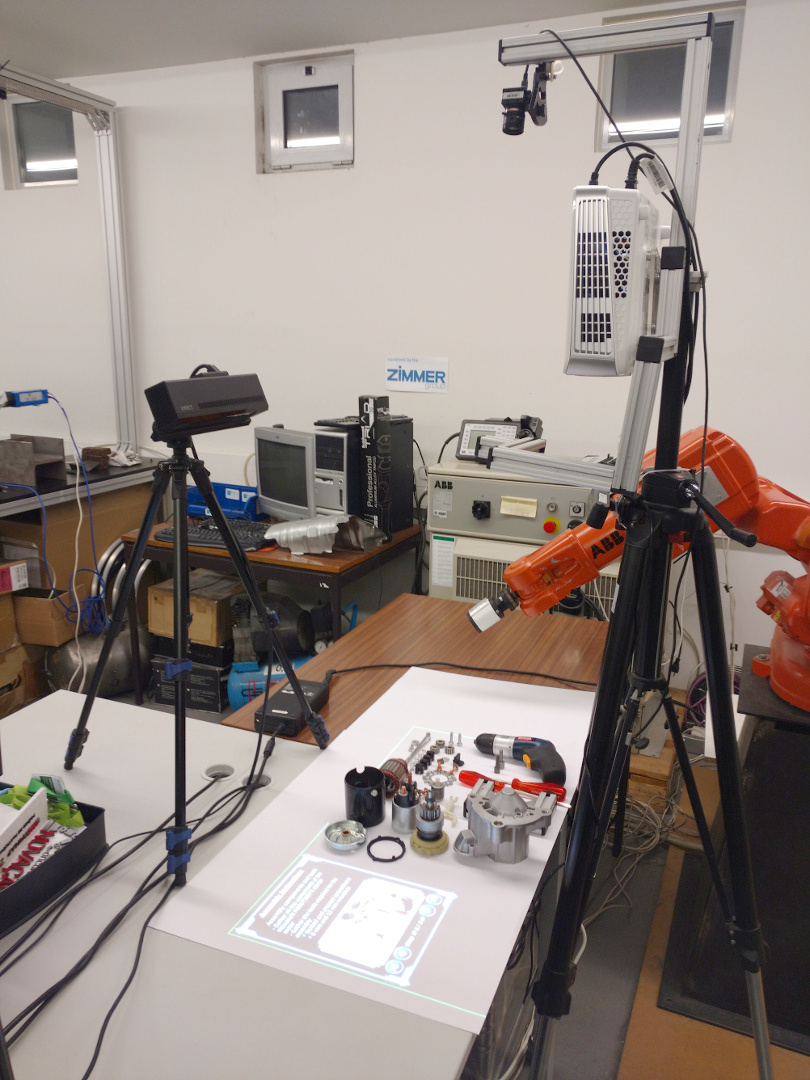
\includegraphics[width=0.4\linewidth]{hardware}
	\caption{Hardware setup}
	\label{fig:hardware}
\end{figure}


\subsection{Training session}

\begin{figure}[H]
	\begin{floatrow}[2]
		\ffigbox[\FBwidth]
		{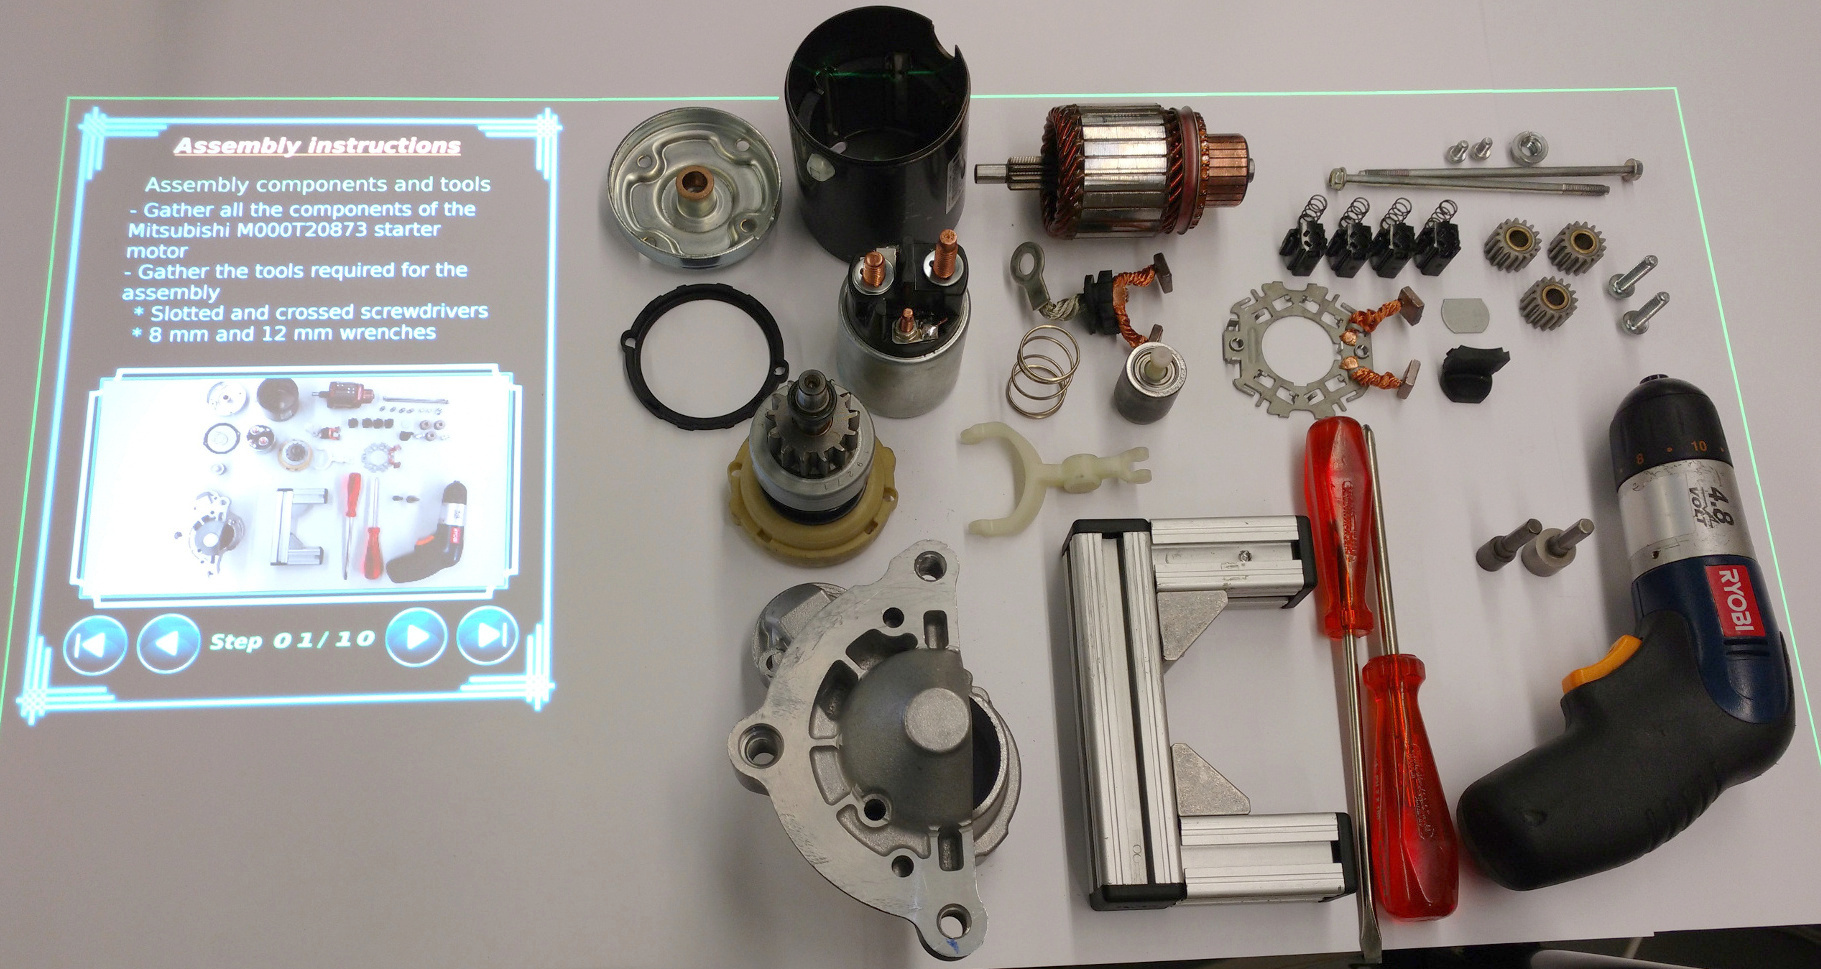
\includegraphics[height=.176\textheight]{assembly-parts}}
		{\caption{Starter engine parts and assembly tools}\label{fig:assembly-parts}}
		\ffigbox[\FBwidth]
		{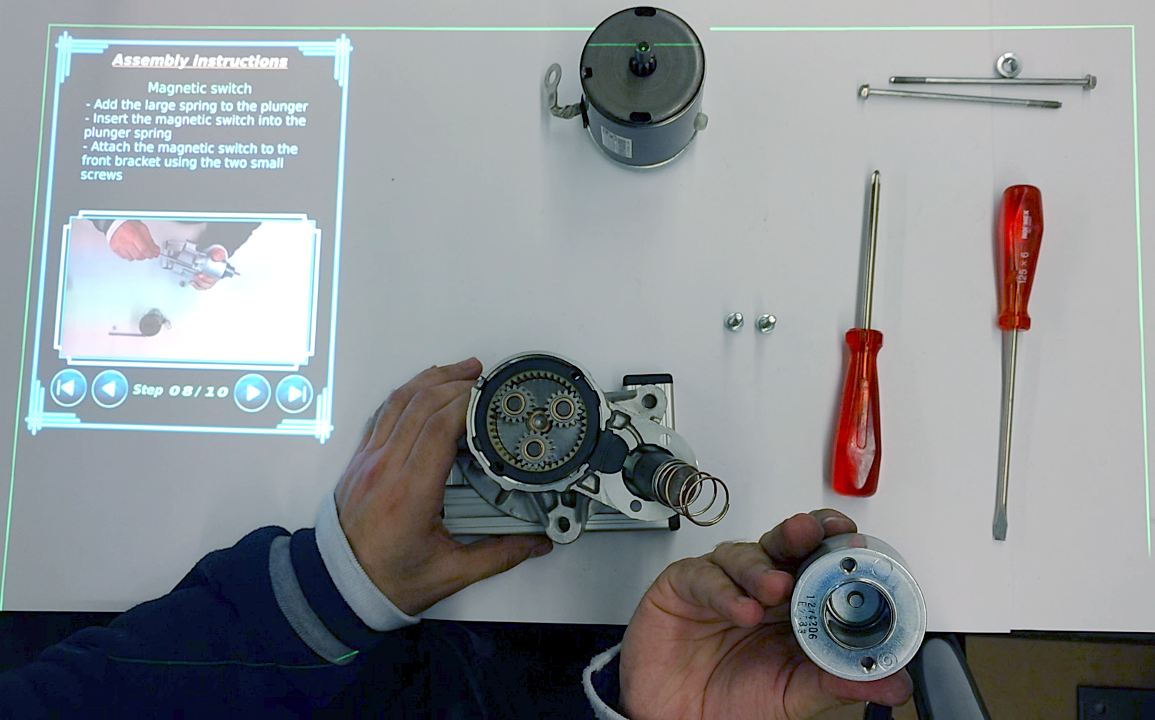
\includegraphics[height=.176\textheight]{assembly}}
		{\caption{Operator assembling starter engine}\label{fig:assembly}}
	\end{floatrow}
\end{figure}

\begin{figure}[H]
	\begin{floatrow}[2]
		\ffigbox[\FBwidth]
		{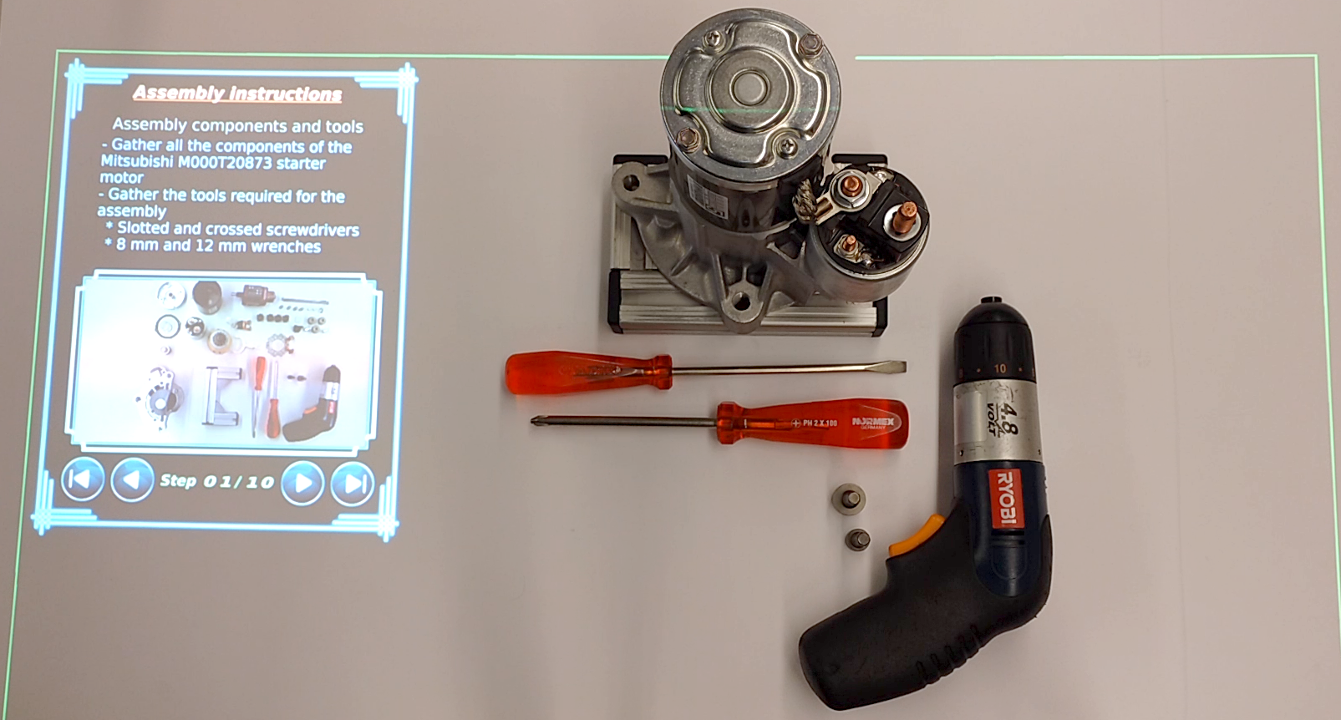
\includegraphics[height=.161\textheight]{assembled-object}}
		{\caption{Starter engine assembled}\label{fig:assembled-object}}
		\ffigbox[\FBwidth]
		{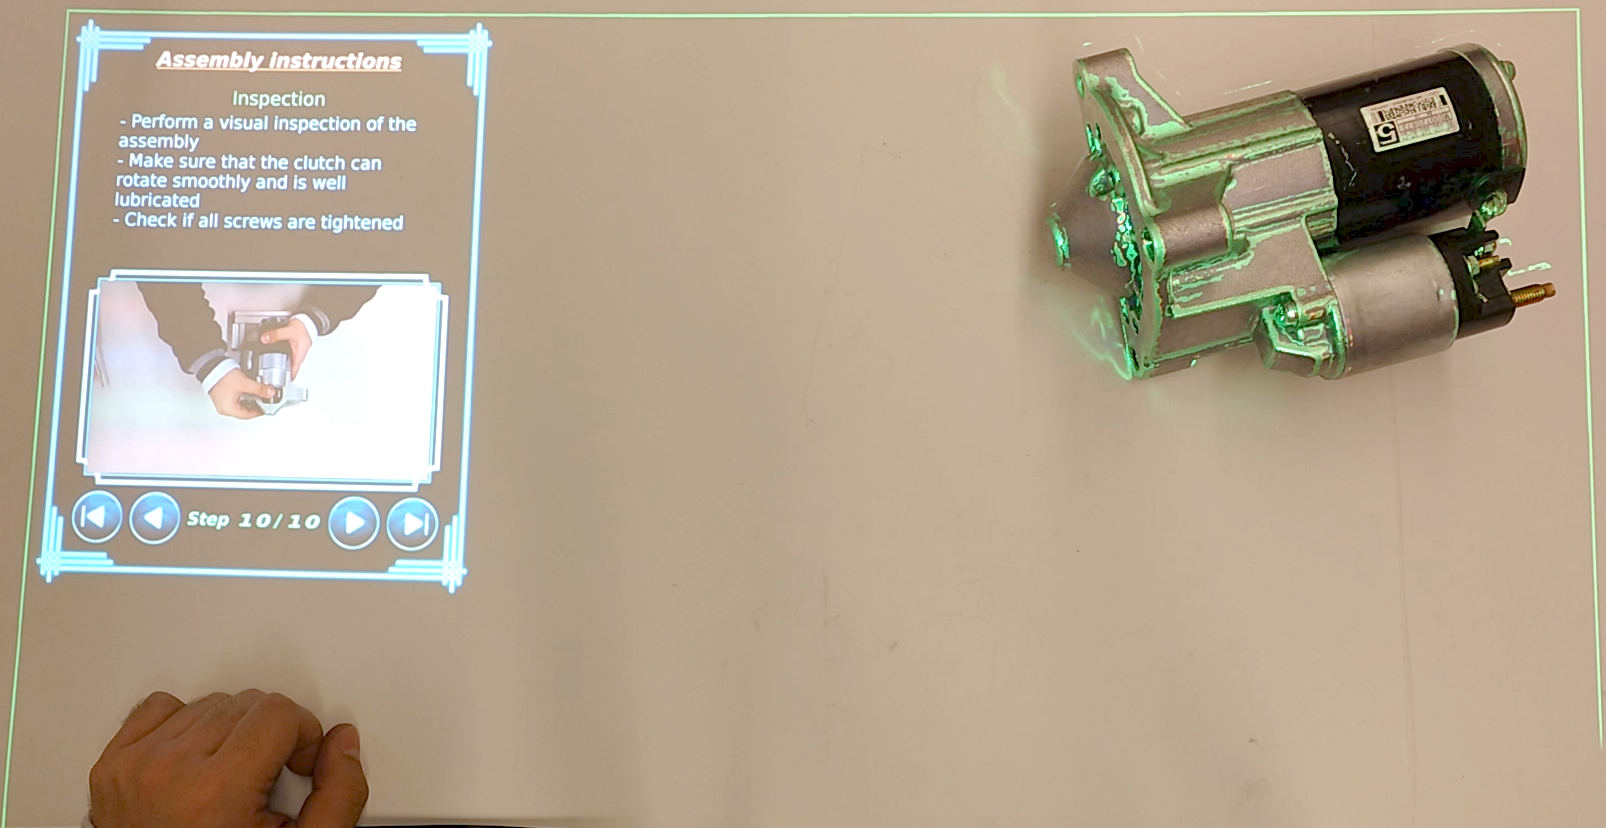
\includegraphics[height=.161\textheight]{projection-mapping-1}}
		{\caption{Projection of the reconstructed 3D model (texture colorized by surface normal curvature)}\label{fig:projection-mapping-1}}
	\end{floatrow}
\end{figure}

\begin{figure}[H]
	\begin{floatrow}[2]
		\ffigbox[\FBwidth]
		{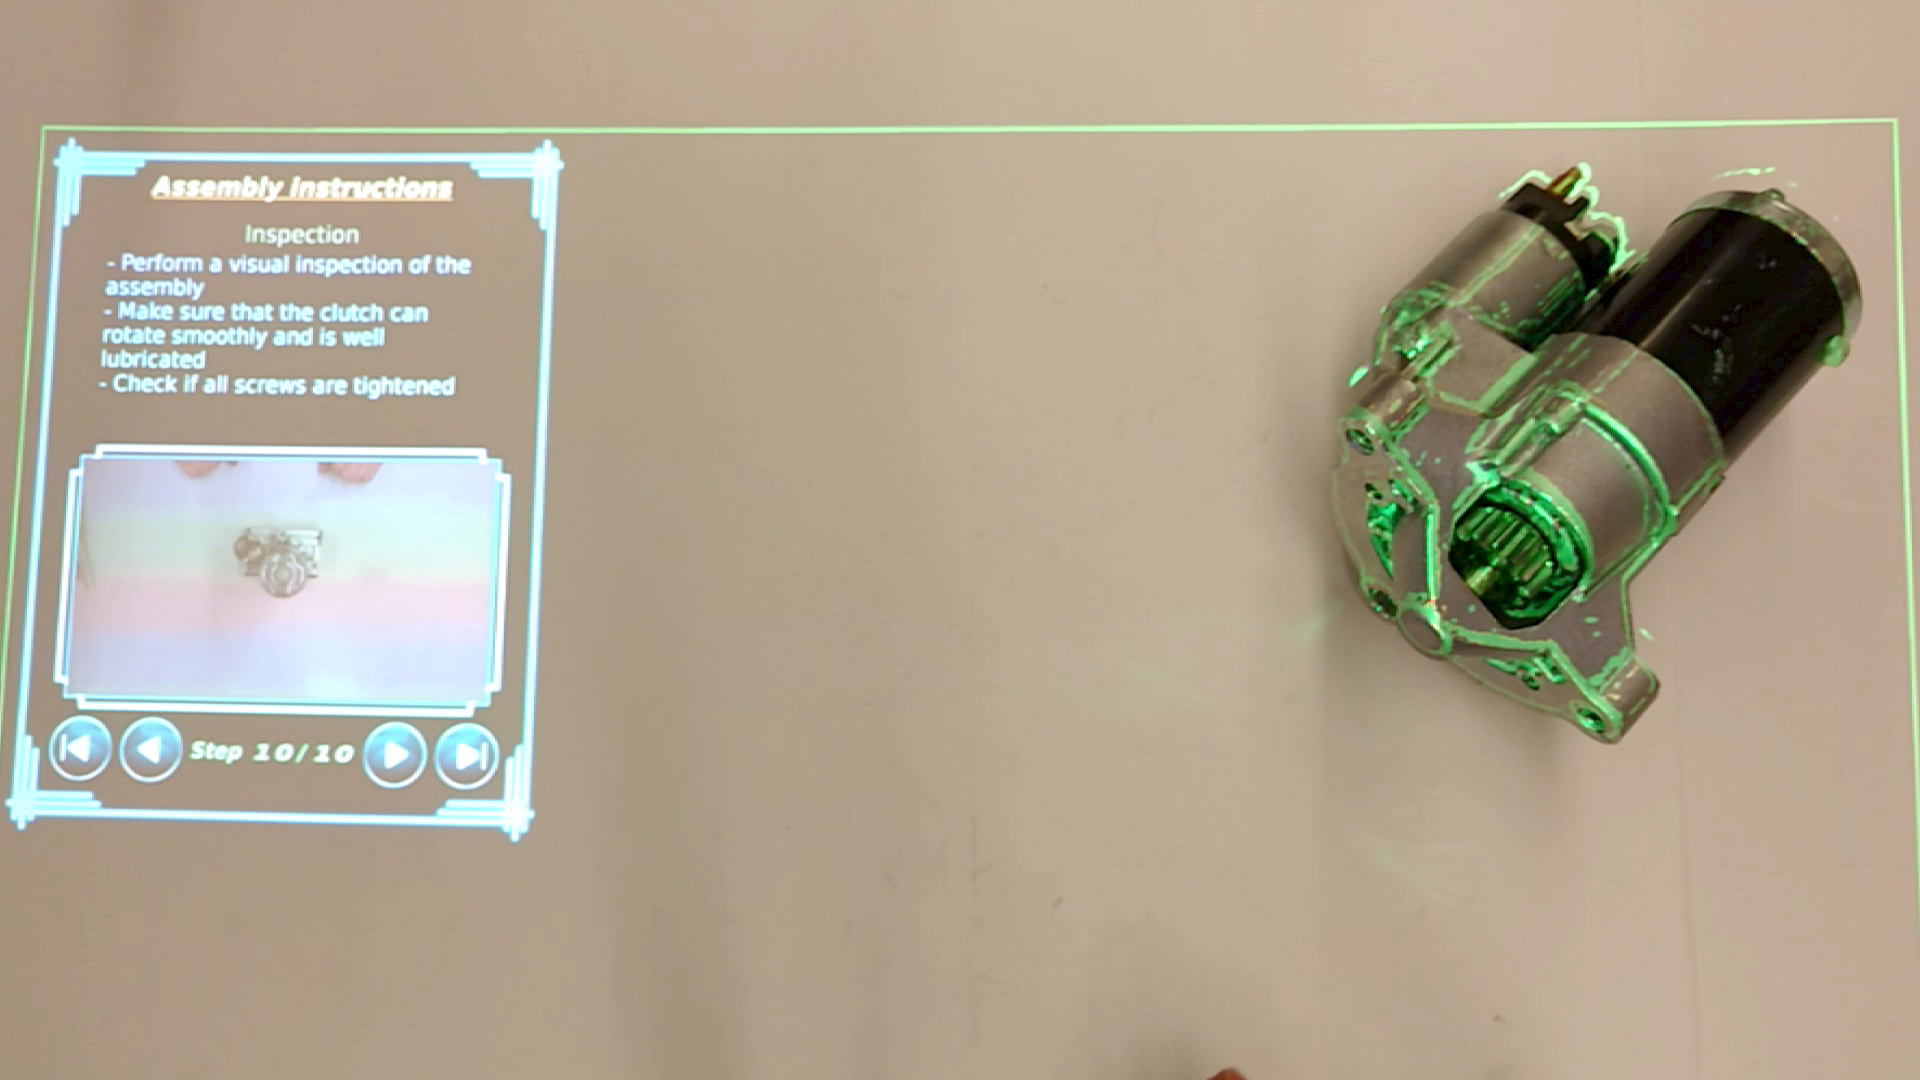
\includegraphics[height=.2\textheight]{projection-mapping-2}}
		{\caption{Object recognition and tracking for update of virtual models pose}\label{fig:projection-mapping-2}}
		\ffigbox[\FBwidth]
		{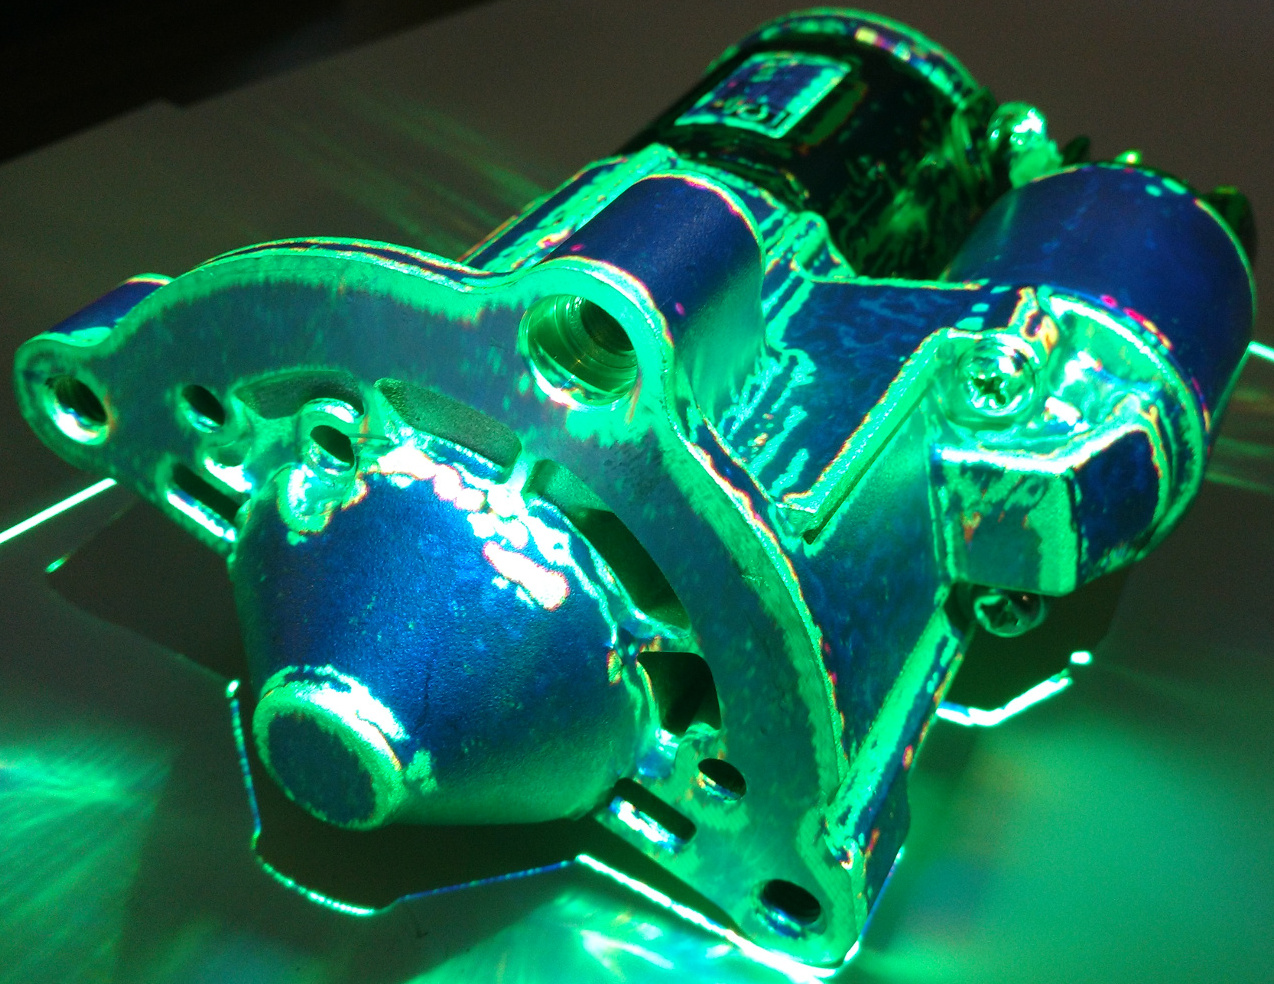
\includegraphics[height=.2\textheight]{projection-mapping-3}}
		{\caption{Detailed view of the assembled object projection}\label{fig:projection-mapping-3}}
	\end{floatrow}
\end{figure}


\begin{figure}[H]
	\begin{floatrow}[4]
		\ffigbox[\FBwidth]
		{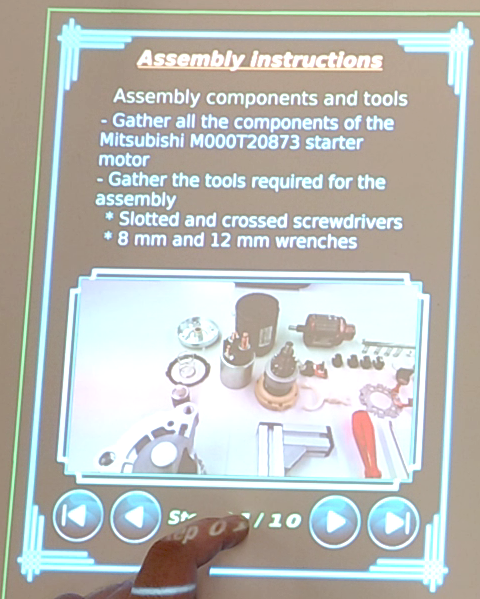
\includegraphics[height=.177\textheight]{interaction-pause}}
		{\caption{Example of video play / pause interaction}\label{fig:interaction-pause}}
		\ffigbox[\FBwidth]
		{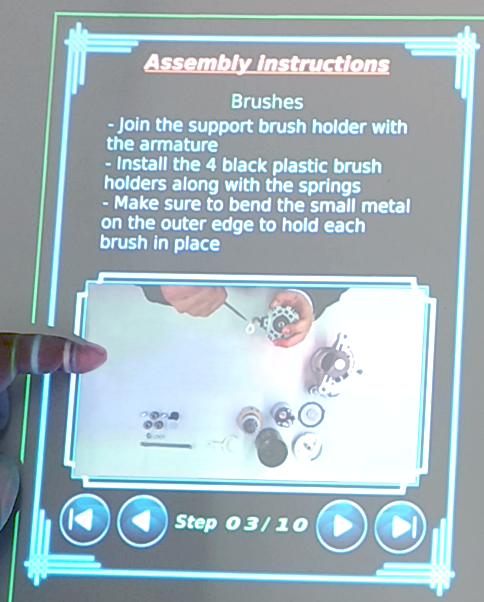
\includegraphics[height=.177\textheight]{interaction-seek}}
		{\caption{Example of video seek interaction}\label{fig:interaction-seek}}
		\ffigbox[\FBwidth]
		{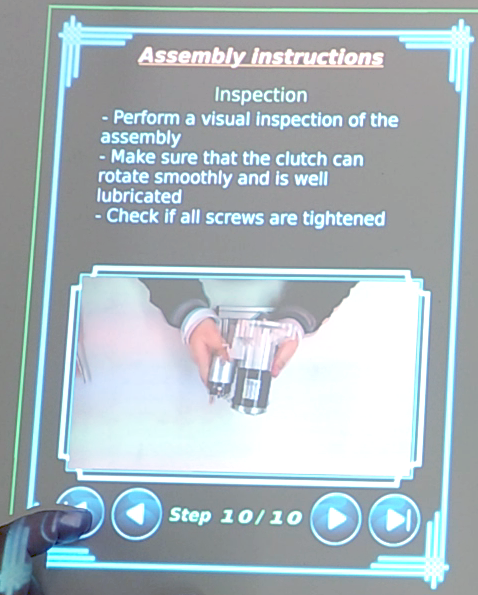
\includegraphics[height=.177\textheight]{interaction-first-0}}
		{\caption{Example of request to move to the first assembly step}\label{fig:interaction-first-0}}
		\ffigbox[\FBwidth]
		{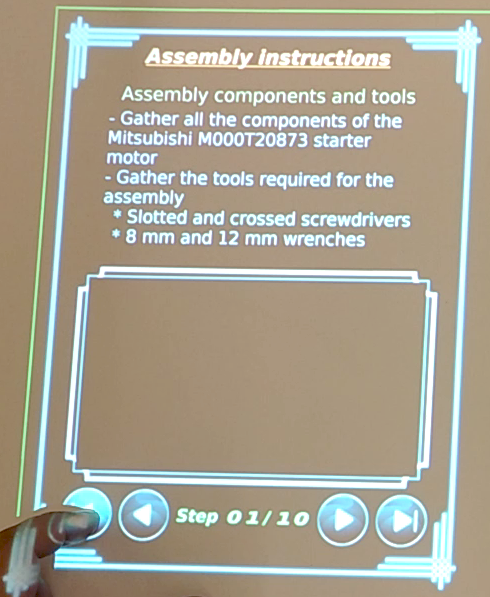
\includegraphics[height=.177\textheight]{interaction-first-1}}
		{\caption{Visual feedback that the request to move to the first assembly step was recognized}\label{fig:interaction-first-1}}
	\end{floatrow}
\end{figure}
